\section*{Ejercicio 1}
Resolviendo la ecuación de onda en una dimensión para únicamente 20 iteraciones, se obtuvieron datos que no mostraban un movimiento como tal, mi hipótesis es que algo conflictuaba entre $\alpha$, $\dd{t}$ y el número de iteraciones. Entonces por prueba y error se logró generar datos para crear un video, el cual se adjunta a este pdf. Se adjunta un frame de dicho video

\begin{figure}[H]
	\centering
	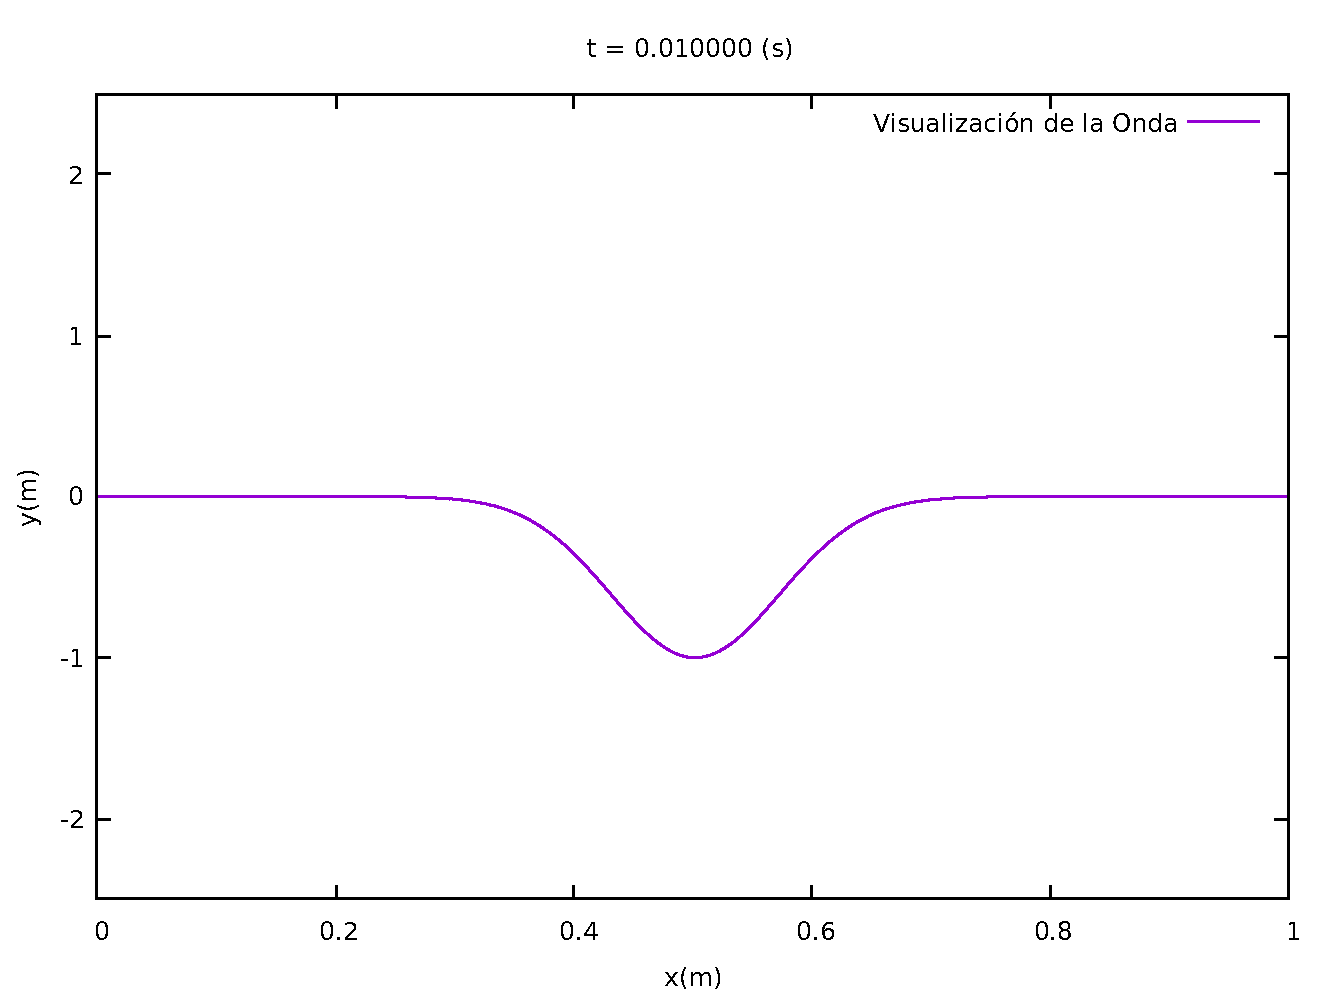
\includegraphics[scale=0.5]{../img/ej7-1.pdf}
	\caption{Frame de la solución a la ecuación de onda en una dimensión.}
	\label{ej7-1}
\end{figure}

\begin{lstlisting}
// Librerias
#include <iostream>
#include <fstream>
#include <cmath>

using namespace std;

double f_cond_ini( double x );
double g_cond_ini( double x );
double w_cond_frontera( double t, double vel );
double z_cond_frontera( double t, double vel );
void output( ostream &of, double *u, double *x, double t, int N );


int main()
{
  int N = 500; //numero de puntos en x
  int out_cada = 20; //output cada no. de iteraciones
  double L = 1.0; //longitud del dominio en x
  double dx = L/N;
  double alfa = 0.5;
  double vel = 2.0; // velocidad de la onda
  double dt = alfa*dx/vel;
  int Niter = 2000; // numero de iteraciones en el tiempo
  double tiempo = 0.0; // lleva la cuenta del tiempo
  ofstream outfile;
  outfile.open( "solucion.dat", ios::out );

  // variables para u
  double *u_nueva = new double[N+1]; // u_{i,j+1}
  double *u       = new double[N+1]; // u_{i,j}
  double *u_vieja = new double[N+1]; // u_{i,j-1}
  double *x       = new double[N+1]; // coordenada x


  // coordenada x
  for( int i=0; i<N+1; i++ )
    x[i] = i*dx;

  // condiciones iniciales u_{i0}
  for( int i=0; i<N+1; i++ )
    u_vieja[i] = f_cond_ini( x[i] );

  // condiciones iniciales u_{i1}
  for( int i=0; i<N+1; i++ )
    u[i] = u_vieja[i] + g_cond_ini( x[i] ) * dt;


  // condicion de frontera
  u[0] = w_cond_frontera( 0.0, vel );
  u[N] = z_cond_frontera( 0.0, vel );


  tiempo += dt;

  // ciclo principal
  for( int j=0; j<=Niter; j++ ){
    for( int i=1; i<N; i++ )
      u_nueva[i] = 2.*(1.-alfa*alfa) * u[i] + alfa*alfa*(u[i-1] + u[i+1]) - u_vieja[i];

    // condicion de frontera
    u_nueva[0] = w_cond_frontera( tiempo + dt, vel );
    u_nueva[N] = z_cond_frontera( tiempo + dt, vel );

    // cambiar instantes de tiempo
    for(int i=0; i<N+1; i++ ){
      u_vieja[i] = u[i];
      u[i]       = u_nueva[i];
    }

    tiempo += dt;

    // output
    if ( j % out_cada == 0 )
      output( outfile, u, x, tiempo, N );

  }



  return 0;
}



void output( ostream &of, double *u, double *x, double t, int N )
{
  for( int i=0; i<N+1; i++ )
    of << t << "\t" << x[i] << "\t" << u[i] << endl;

  of << endl << endl;
}



double f_cond_ini( double x )
{
  double L = 1.0; // longitud de la cuerda
  //return sin(4*2.*M_PI*x);
  //return exp(-100*pow(x-L/2,2));
  return 0.0;
}


double g_cond_ini( double x )
{
  double L = 1.0; // longitud de la cuerda
  //return 10*exp(-100*pow(x-L/2,2));
  return 0.0;
}


double w_cond_frontera( double t, double vel )
{
  return exp(-100*(0 - vel*t - 0.5)*(0 - vel*t - 0.5));
}


double z_cond_frontera( double t, double vel )
{
  return exp(-100*(1 - vel*t - 0.5)*(1 - vel*t - 0.5));
}
\end{lstlisting}

\section*{Ejercicio 2}
Al programa ya mostrado, únicamente se le agrega la condición inicial en la velocidad y el número de iteraciones a $20$. 

\begin{figure}[H]
	\centering
	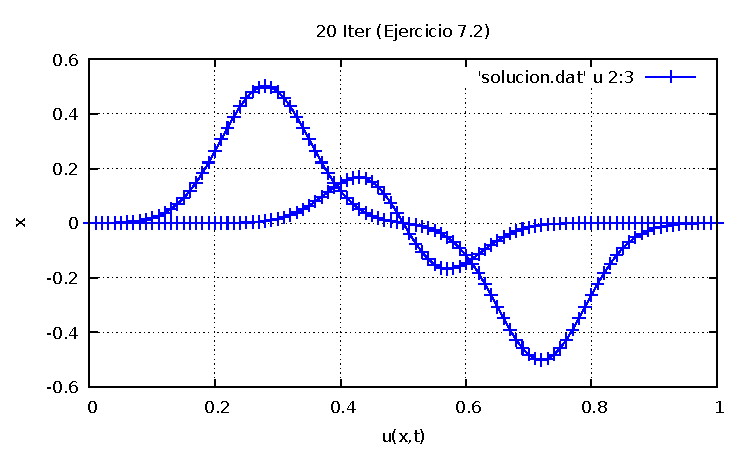
\includegraphics[scale=1]{../img/ej7-2.pdf}
	\caption{Los "frames" superpuestos en una gráfica.}
	\label{ej7-2}
\end{figure}


\begin{lstlisting}
double g_cond_ini( double x, double vel )
{
  double L = 1.0; // longitud de la cuerda

  return -200*vel*(x - 0.5)*exp(-100*(x - 0.5)*(x - 0.5));
}
\end{lstlisting}

\section*{Ejercicio 3}
Tomando las constantes $\alpha$ y $\beta$ como $\pm 1$ se manipulan las condiciones iniciales y de frontera manteniendo el signo de la constante en todas. De modo que las funciones de condiciones de frontera e iniciales son

\begin{lstlisting}
double f_cond_ini( double x, double vel )
{
  double L = 1.0; // longitud de la cuerda

  return exp(-100*(x-0.75)*(x-0.75))+exp(-100*(x-0.25)*(x-0.25)); // interferencia constructiva
  //return exp(-100*(x-0.75)*(x-0.75))-exp(-100*(x-0.25)*(x-0.25)); // interferencia destructiva
}


double g_cond_ini( double x, double vel )
{
  double L = 1.0; // longitud de la cuerda

  return -200*vel*(x-0.75)*exp(-100*((x-0.75)*(x-0.75)))+200*vel*(x-0.25)*exp(-100*((x-0.25)*(x-0.25))); // interferencia constructiva
  //return -200*vel*(x-0.75)*exp(-100*((x-0.75)*(x-0.75)))-200*vel*(x-0.25)*exp(-100*((x-0.25)*(x-0.25))); // interferencia destructiva
}


double w_cond_frontera( double t, double vel )
{
  return  exp(-100*((0+vel*t)-0.75)*((0+vel*t)-0.75))+exp(-100*((0-vel*t)-0.25)*((0-vel*t)-0.25)); // interferencia constructiva
  //return  exp(-100*((0+vel*t)-0.75)*((0+vel*t)-0.75))-exp(-100*((0-vel*t)-0.25)*((0-vel*t)-0.25)); // interferencia destructiva
}


double z_cond_frontera( double t, double vel )
{
  return  exp(-100*((1+vel*t)-0.75)*((1+vel*t)-0.75))+exp(-100*((1-vel*t)-0.25)*((1-vel*t)-0.25)); // interferencia constructiva
  //return  exp(-100*((1+vel*t)-0.75)*((1+vel*t)-0.75))-exp(-100*((1-vel*t)-0.25)*((1-vel*t)-0.25)); // interferencia destructiva
}
\end{lstlisting}

Con estas modificaciones se tienen las siguientes gráficas justo antes de que las ondas se encuentren.

\begin{figure}[H]
	\centering
	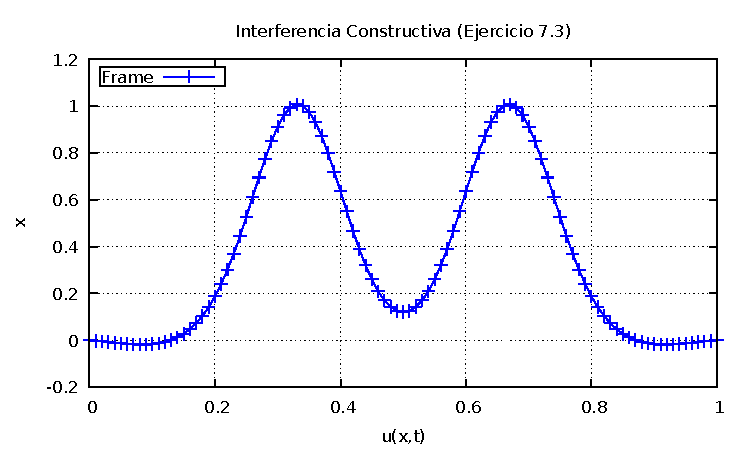
\includegraphics[scale=1]{../img/ej7-3c.pdf}
	\caption{Interferencia constructiva.}
	\label{ej7-3c}
\end{figure}


\begin{figure}[H]
	\centering
	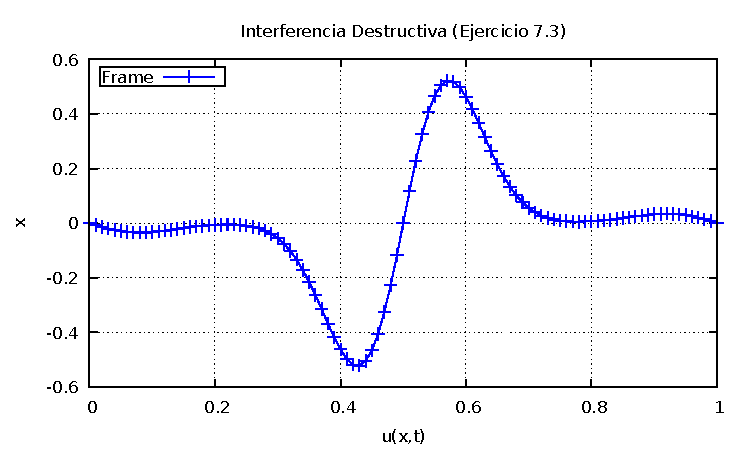
\includegraphics[scale=1]{../img/ej7-3d.pdf}
	\caption{Interferencia destructiva.}
	\label{ej7-3d}
\end{figure}












































%%%%%%%%%%%%%%%5555
